\documentclass[tikz]{standalone}
\usepackage{tikz}
\usetikzlibrary{arrows.meta, positioning, shapes.geometric}

\tikzset{
  io/.style      = {trapezium, trapezium left angle=70, trapezium right angle=110,
                    draw, text width=3.4cm, minimum height=1.1cm, align=center},
  process/.style = {rectangle, rounded corners=3pt, draw, text width=4.0cm,
                    minimum height=1.15cm, align=center},
  data/.style    = {rectangle, draw, dashed, text width=4.0cm, minimum height=1.0cm,
                    align=center},
  support/.style = {rectangle, draw, text width=3.5cm, minimum height=1.1cm,
                    align=center, fill=gray!10},
  flow/.style    = {-{Stealth[length=2.5mm]}, very thick}
}

\begin{document}
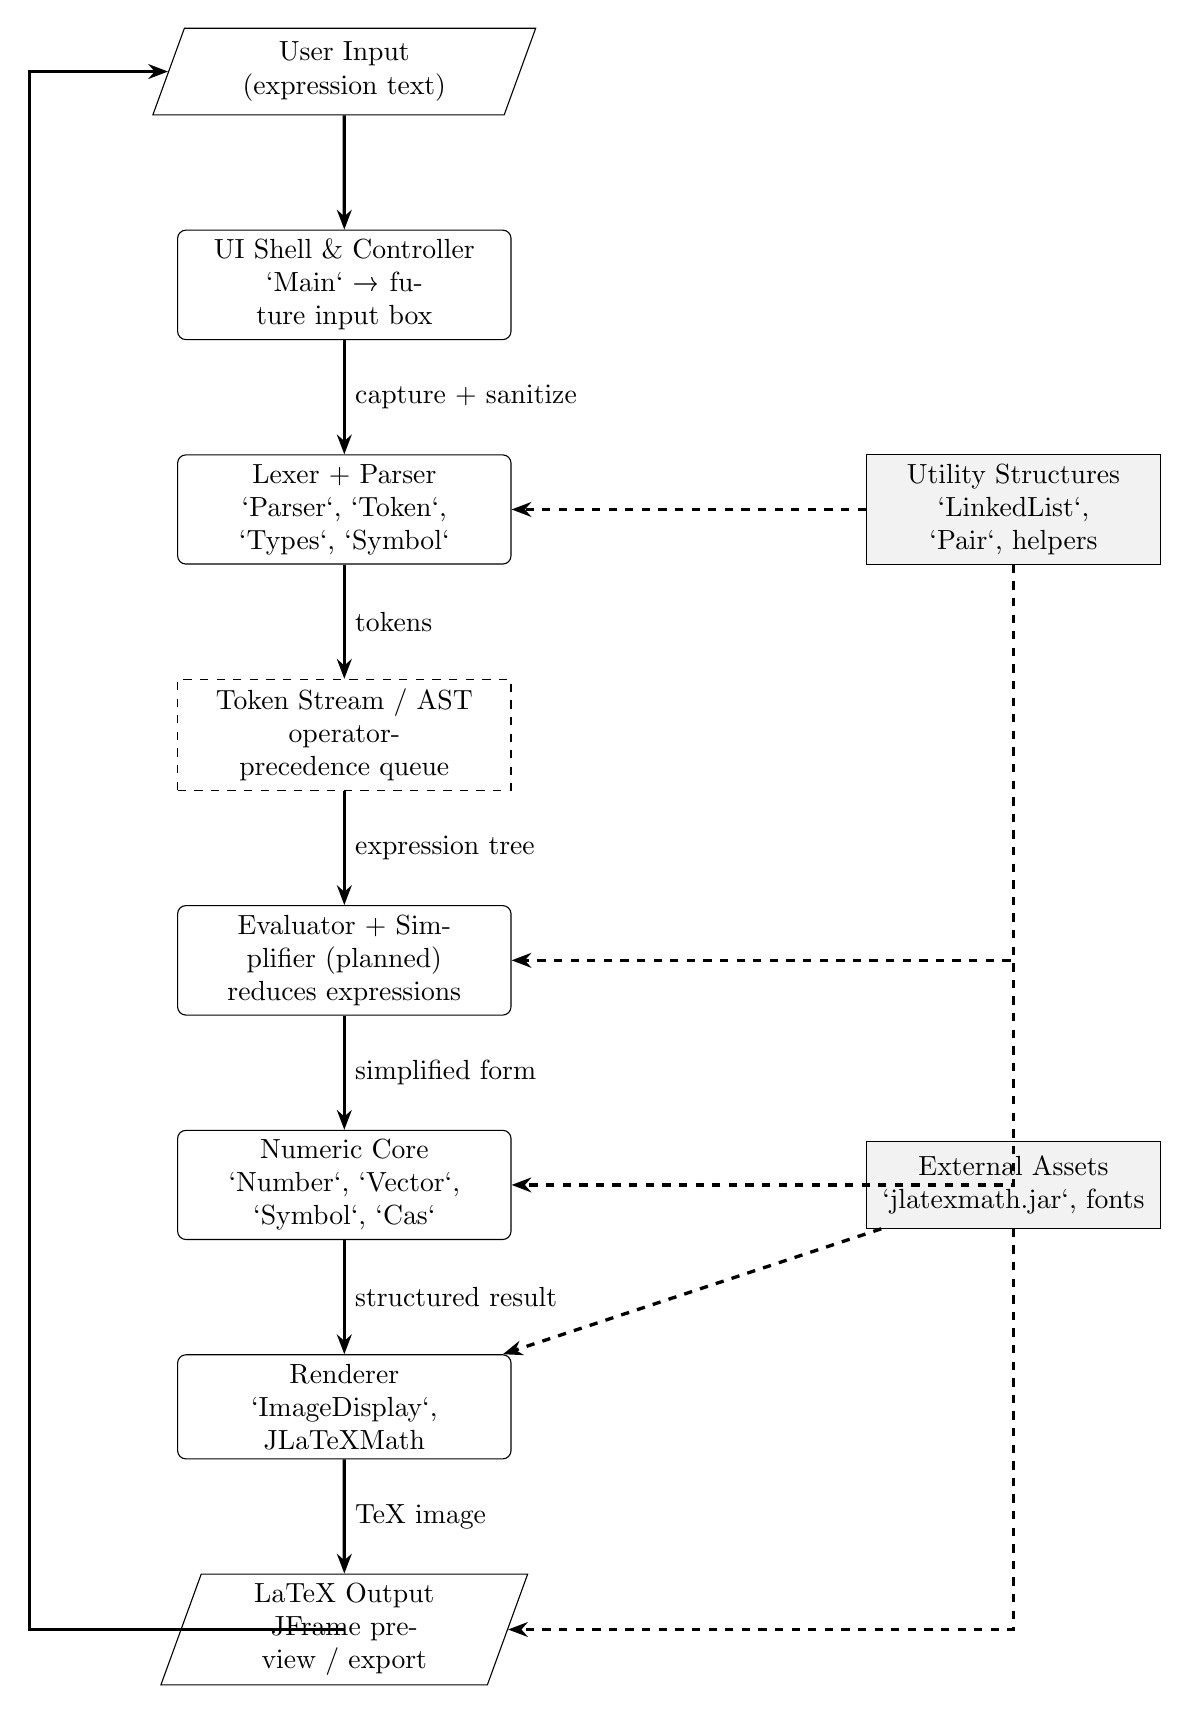
\begin{tikzpicture}[node distance=1.45cm and 2.6cm]
  \node[io]      (userIn)  {User Input \\ (expression text)};
  \node[process] (ui)      [below=of userIn]
                   {UI Shell \& Controller\\`Main` \textrightarrow{} future input box};
  \node[process] (parser)  [below=of ui]
                   {Lexer + Parser\\`Parser`, `Token`, `Types`, `Symbol`};
  \node[data]    (ast)     [below=of parser]
                   {Token Stream / AST\\ operator-precedence queue};
  \node[process] (eval)    [below=of ast]
                   {Evaluator + Simplifier (planned)\\reduces expressions};
  \node[process] (numeric) [below=of eval]
                   {Numeric Core\\`Number`, `Vector`, `Symbol`, `Cas`};
  \node[process] (render)  [below=of numeric]
                   {Renderer\\`ImageDisplay`, JLaTeXMath};
  \node[io]      (display) [below=of render]
                   {LaTeX Output\\JFrame preview / export};

  \node[support] (utils)   [right=4.5cm of parser]
                   {Utility Structures\\`LinkedList`, `Pair`, helpers};
  \node[support] (lib)     [right=4.5cm of numeric]
                   {External Assets\\`jlatexmath.jar`, fonts};

  \draw[flow] (userIn) -- (ui);
  \draw[flow] (ui) -- node[right]{capture + sanitize} (parser);
  \draw[flow] (parser) -- node[right]{tokens} (ast);
  \draw[flow] (ast) -- node[right]{expression tree} (eval);
  \draw[flow] (eval) -- node[right]{simplified form} (numeric);
  \draw[flow] (numeric) -- node[right]{structured result} (render);
  \draw[flow] (render) -- node[right]{TeX image} (display);
  \draw[flow] (display) |- ++(-4,0) |- (userIn);

  \draw[flow, dashed] (utils) -- (parser);
  \draw[flow, dashed] (utils) |- (eval);
  \draw[flow, dashed] (utils) |- (numeric);

  \draw[flow, dashed] (lib) -- (render);
  \draw[flow, dashed] (lib) |- (display);
\end{tikzpicture}
\end{document}
